\documentclass[oneside, final, 14pt,  a4paper]{extreport}
% TODO: 1. Длинные заголовки при переносе строки продолжаются под цифрами. Т.е. не
%          начало текста не выровнено
% ----------------------------- БАЗОВЫЕ НАСТРОЙКИ  -----------------------------

\documentclass[oneside, final, 14pt,  a4paper]{extreport}    % Класс документа. Чаще всего использует его
\usepackage[T2A]{fontenc}
\usepackage[utf8]{inputenc}                        % Кодировка utf8x для linux
\usepackage[english,russian]{babel}                % Переносы и прочее для русского и английского
\usepackage{cmap}                                  % Нормальные русские символы в получаемом pdf
\usepackage[linktocpage=true]{hyperref}            % Гиперссылки
\usepackage{indentfirst}                           % Красная строка для первых абзацев
\usepackage{mathtools}
\usepackage{tabularx}                              % Много табличной боли и магии
\usepackage[pdftex]{graphicx}                      % Для вставки картинок
\usepackage{titlesec}                              % Для настройки названий глав, разделов итп
\usepackage{titletoc}                              % Для настройки оглавления
\usepackage{enumitem}                              % Для настройки списков
\usepackage{flafter}                               % Плавающие элементы встречаются после ссылки на них
\usepackage{caption}                               % Настройка подписей плавающих элементов
\usepackage{setspace}                              % Для настройки интервалов
\usepackage{csquotes}
\usepackage{chngcntr}                              % Чтоб настроить сквозную нумерацию
\usepackage{lastpage}                              % Получить количество страниц
\usepackage[figure,table]{totalcount}              % Получить количество рисунков и таблиц
\usepackage{svg}                                   % Использование SVG в рисунках

% Библиография
\usepackage[
    backend=biber,
    sorting=none,                                  % Сортировка в порядке цитирования
	style=gost-numeric,
	language=auto,                                 % Автовыбор стиля, напр. писать [et al] вместо [и др]
	autolang=other                                 % для англоязычных публикаций (langid={english})
] {biblatex}

\linespread{1.3}                                   % Полуторный интервал

% Настройка полей
\usepackage{geometry}
\geometry{left=3cm}
\geometry{right=1cm}
\geometry{top=1.5cm}
\geometry{bottom=2cm}


\sloppy                                           % Избегать залезания строк на поля (надо?)
\setlength\parindent{1.5cm}                       % Отступ красной строки

\newcommand{\nf}{\normalfont}

% Для tabularx:
\newcolumntype{Y}{>{\centering\arraybackslash}X} % Растянутый столбец (как X) с выравниванием по центру
\newcolumntype{P}{>{\raggedleft\arraybackslash}X}% Растянутый столбец (как X) с выравниванием по справа

% ----------------------------- НАСТРОЙКИ ЗАГЛАВИЙ -----------------------------
%% Отступ 1.5 слева (как у красной строки)t
% Нет точки между номером и названием
% Интервал между подзаголовками 1.5
% Интервал между заголовком и текстом 2*1.5
% Поддержка приложений

% Глава
\titleformat{\chapter}
	[block]                % Shape. block убирает перенос заглвания на новую строку
    {\normalfont}          % Format. Собственно, стиль
    {\thechapter}          % Label. Номер главы.
    {8pt}                  % Sep. Пробел между номером и главой (TODO: уточнить)
    {}                     % before-code. Код перед названием
\titlespacing*{\chapter}
	{1.5cm}                % Левый отступ (как у красной строки)
	{18pt}                 % Верхний отступ, 1.5 интервал
	{18pt}                 % Нижний отступ, 1.5 интервал

% Раздел
\titleformat{\section}
	{\normalfont}
	{\thesection}
	{8pt}{}
\titlespacing*{\section}
	{1.5cm}{18pt}{18pt}

% Подраздел
\titleformat{\subsection}
	{\normalfont}
	{\thesubsection}
	{8pt}{}
\titlespacing*{\subsection}
	{\parindent}{18pt}{18pt}

% Глава без номера (введение, заключение и т.п.)
\newcommand{\nnchapter}[1]
{
	\chapter*{#1}
	\addcontentsline{toc}{chapter}{#1}
}

% Приложения
% Использовать \chapter{} для создания приложений
% Очень грязный хак, но работает
\newcommand{\StartAppendix}
{
	\setcounter{chapter}{0}
}

\renewcommand{\appendix}[1]
{
	\newpage
	\stepcounter{chapter}
	\newcommand{\theappendix}{ПРИЛОЖЕНИЕ \MakeUppercase{\asbuk{chapter}}}
	\addcontentsline{toc}{chapter}{\texorpdfstring{\theappendix} ~--- #1}
	\begin{center}
		\theappendix\\
		{#1}
	\end{center}
}

% Расстояние между заглавиями и текстом должно быть 2 полуторных интервала,
% а расстояние между заглавиями - один полуторный интервал.
% Не придумал ничего лучше, кроме как вставлять вручную
\newcommand{\aftertitle}{\vskip 18pt}

% ----------------------------- НАСТРОЙКИ СОДЕРЖАНИЯ ---------------------------
% Нет выделения жирным
% Все с одним уровнем отступа
% Поддержка приложений

% Главы
\titlecontents{chapter}
	[0em] {}
	{\thecontentslabel~}{}
	{\titlerule*[1pc]{.}\contentspage}

% Разделы
\titlecontents{section}
	[0em] {}
	{\thecontentslabel~}{}
	{\titlerule*[1pc]{.}\contentspage}

% Подразделы
\titlecontents{subsection}
	[0em] {}
	{\thecontentslabel~}{}
	{\titlerule*[1pc]{.}\contentspage}

% Заголовок
\addto\captionsrussian{
	\renewcommand{\contentsname} {СОДЕРЖАНИЕ}
}

%-------------------------------- НАСТРОЙКИ СПИСКОВ ----------------------------
% Маркерный список
\setlist[itemize]{
	label=-,                  % Дефис в каяестве маркера
	leftmargin=1.5cm,         % Текст в списке выравнен по красной строке
	itemindent=15pt,          % Маркер выравнен по красной строке, т.е. первая строка чуть сдвинута на размер маркера
	nosep                     % Убираем интервал между пунктами списков
}

% Числовой
\setlist[enumerate]{
    leftmargin=1.5cm,
    nosep
}
\setlist[enumerate,1]{
	label=\arabic*),
	itemindent=18pt,
}
\setlist[enumerate,2]{
	label=\arabic{enumi}.\arabic*),
	itemindent=30pt,
}
% NOTE: сейчас поддерживается только два уровня вложенности, если нужно больше -
% нужно добавить

%--------------------------- НАСТРОЙКИ РИСУНКОВ И ТАБЛИЦ -----------------------
% Рисунки подписываются "Рисунок N - ..." по центру
% Таблицы подписываются "Таблица N - ..." с левого края

\captionsetup[figure]{
	name=Рисунок,
	labelsep=endash,
	justification=centering,
	belowskip=-17pt,aboveskip=0pt,
	font={stretch=1.3}
}
\captionsetup[table]{name=Таблица, labelsep=endash, justification=raggedright, singlelinecheck=false}

% Сквозная нумерация таблиц, рисунков и формул
\counterwithout{figure}{chapter}
\counterwithout{table}{chapter}
\counterwithout{equation}{chapter}
\pdfimageresolution=150

%\setlength{\belowcaptionskip}{-14pt}

%-------------------------------- БИБЛИОГРАФИЯ ---------------------------------

\addbibresource{bibliography.bib}

\begin{document}

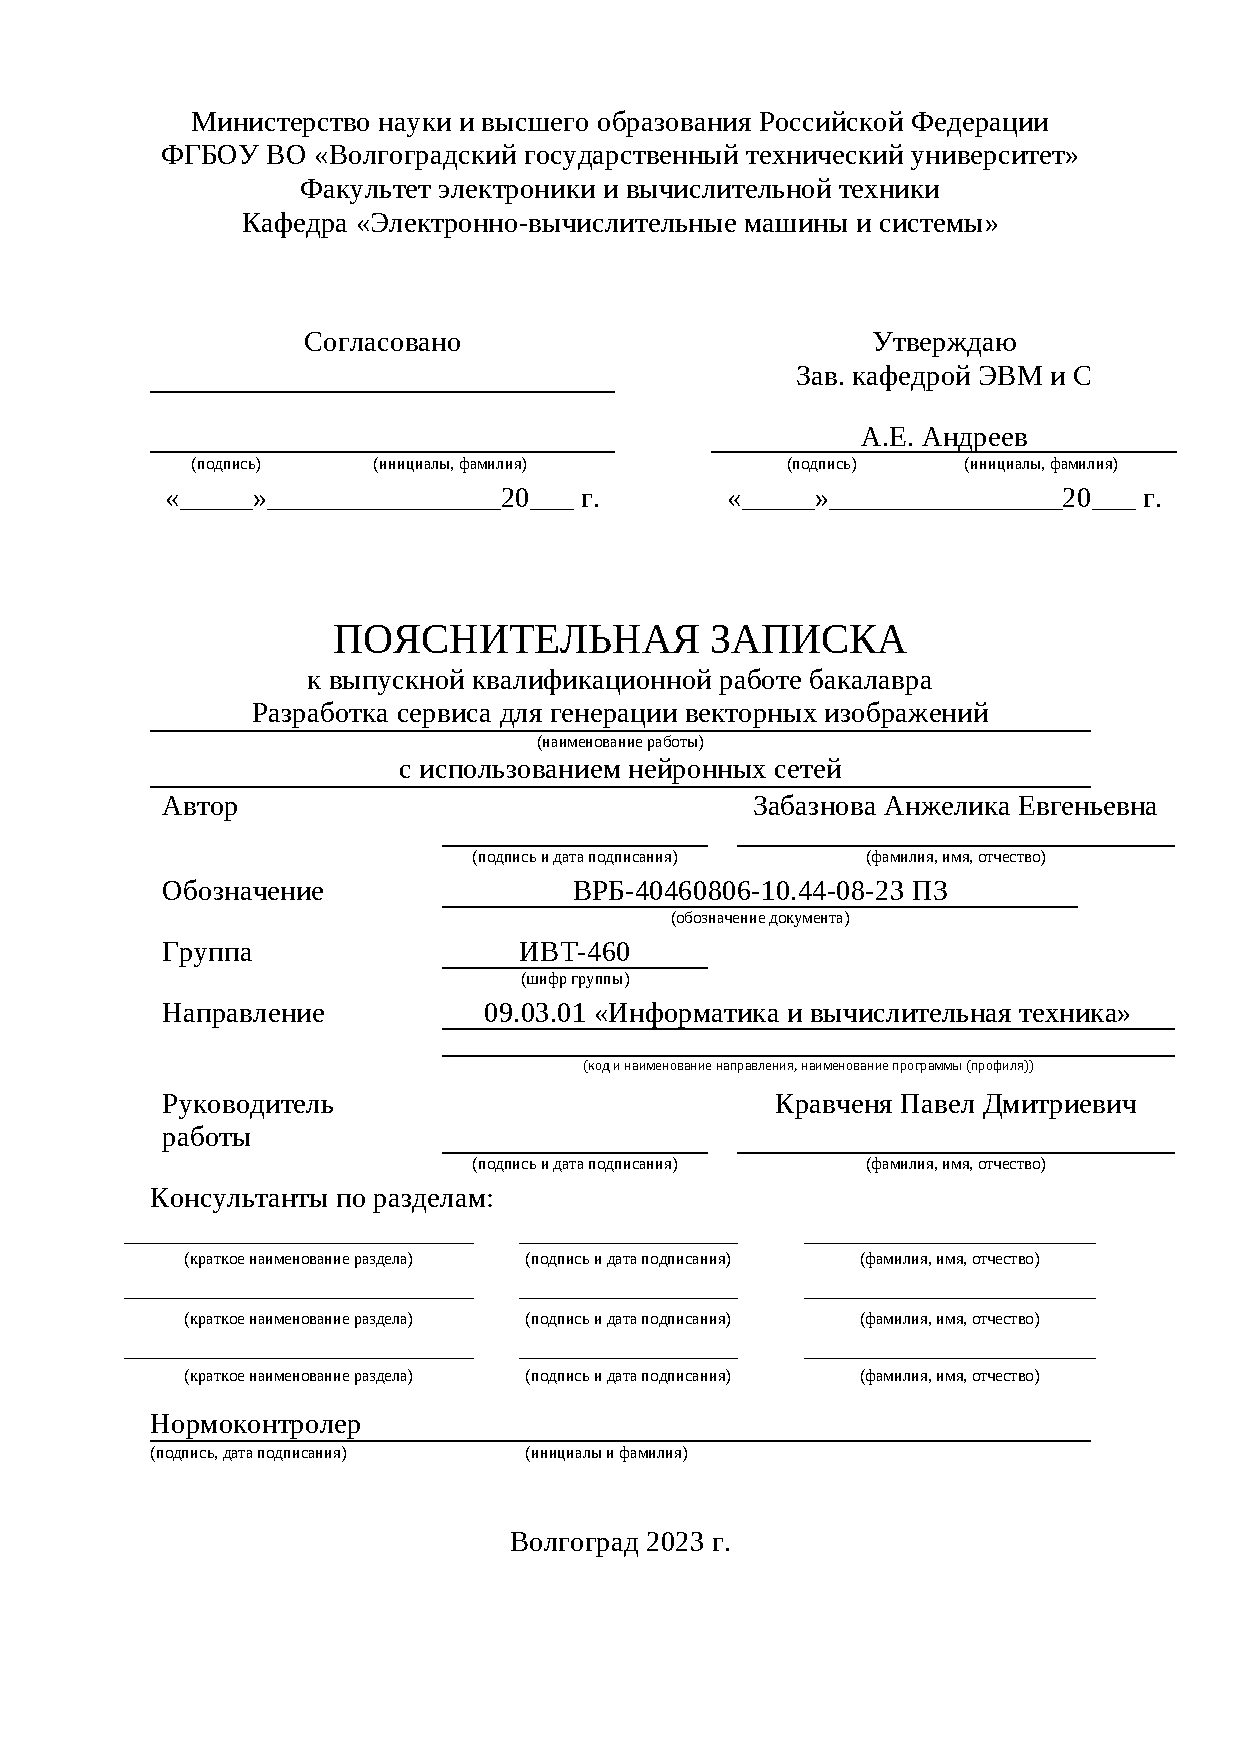
\includepdf[pages=-]{title/title.pdf}
\begin{center}
	АННОТАЦИЯ
\end{center}

TODO: Аннотация

Данная работа состоит из \pageref{LastPage} страниц, \totalfigures ~рисунков и
\totaltables ~таблиц.

\begin{center}
	ABSTRACT
\end{center}

TODO: Abstract in English

This paper consists of \pageref{LastPage} pages and includes \totalfigures ~figures and
\totaltables ~tables.

\tableofcontents
\nnchapter{ВВЕДЕНИЕ}
\aftertitle

В настоящее время в мире генерируется большой объем новостной информации. Изучение и анализ новостей является востребованной задачей в различных областях бизнеса и науки. Выявление трендов, анализ популярных новостей и другие задачи применяются в таких областях, как социологические исследования, маркетинговые исследования, экономические и финансовые прогнозы и другое.

Из-за большого объема новостной информации, который генерируется ежедневно, людям, которые имеют потребность в изучении новостей, затруднительно или невозможно производить их анализ вручную. Поэтому актуальной является задача разработки системы, позволяющей автоматизировать обработку новостных данных.

Целью данной работы является автоматизация процесса получения и анализа новостей: определение их характеристик, определение семантического сходства и взаимной корреляции.

Для выполнения цели были поставлены следующие задачи:
\begin{enumerate}
    \item произвести аналитический обзор предметной области с целью выяснения актуального состояния, существующих решений, их преимуществ и недостатков, существующих подходов к решению поставленной цели;
    \item спроектировать веб-сервис для получения и анализа новостей;
    \item реализовать веб-сервис для получения и анализа новостей;
    \item протестировать веб-сервис и произвести эксперименты по анализу новостей.
    \item произвести исследование новостей с использованием разработанного сервиса, осуществить поиск корреляции новостей с ценами финансовых инструментов.
\end{enumerate}

\chapter{АНАЛИЗ ПРЕДМЕТНОЙ ОБЛАСТИ}
\aftertitle

Задачу кластеризации текста можно разделить на два этапа:
\begin{enumerate}
    \item формирование эмбедингов текстов, т.е. перевод текстов в векторное представление, которое может быть использовано в различных алгоритмах кластеризации;
    \item кластеризация полученных эмбедингов с помощью тех или иных алгоритмов кластеризации.
\end{enumerate}

TODO: Возможно, эту секцию можно будет переписать, чтобы делать обзор не по статьям, а по методам, которые могут рассматриваться более, чем в одной статье.

В работе \cite{compare-text-clustering-sokolov} произведено сравнение следующих методов кластеризации текстовой информации: метод k-средних, алгоритм спектральной кластеризации, алгоритм агломеративной кластеризации и самоорганизующаяся карта Кохонена. В качестве данных использовалась коллекция новостей на русском языке. Для получения эмбедингов текста применялся алгоритм "мешок слов" ("bag of words"). В этой модели весь текст представлен одним вектором, хранящим информацию о количественном составе каждого слова в тексте. Недостатком данного подхода является отсутствие семантических связей между словами в тексте. В результате сравнения, алгоритмы показали достаточно близкую точность работы между собой, но, в среднем, самоорганизующиеся карты Кохонена оказались лучше других. Используемые алгоритмы сильно зависят от настройки гиперпараметров. Оптимальные параметры подбирались автоматически.

TODO: написать про эти методы? k-means понятно, остальные непонятно.

TODO: еще применяют метрику TF-IDF.

В работе \cite{method-text-clustering-andreev} дается обзор различных методов кластеризации, такие как: метод k-средних, suffix tree clustering, иерархические методы single link, complete link, group average, самоорганизующаяся карты Кохонена и сети ART (TODO: ???).

\chapter{АРХИТЕКТУРА И ПРОЕКТИРОВАНИЕ}

\textbf{TODO: Дописать вторую главу ВБР (12-15 страниц): модель, архитектура и проектирование сервиса, архитектурное взаимодействие с БД и ее плагинами.}


В данной главе рассматривается архитектура и проектирование системы анализа новостей. Проектирование системы основано на анализе рассмотренных решений и алгоритмов.

\section{Формулирование требований к системе анализа новостей}
В рамках данной работы разрабатывается сервис, позволяющий анализировать семантическое сходство пользовательских запросов и новостей за определенный промежуток времени с использованием нейронных сетей.

Были сформулированы следующие требования к системе:

\begin{enumerate}
    \item функциональные требования:
    \begin{enumerate}
        \item сервис должен предоставлять пользователю REST API для взаимодействия с сервисом;
        \item сервис должен предоставлять возможность семантического поиска новостей;
        \item сервис должен предоставлять возможность определять основные темы новостей за заданный промежуток времени;
        \item сервис должен предоставлять возможность расчёта корреляции количества новостей по заданным темам с предоставленными пользователем числовыми рядами;
    \end{enumerate}
    \item Требования к окружению:
    \begin{enumerate}
        \item Сервис должен работать на серверах под управлением ОС Linux;
        \item Сервис должен использовать GPU для ускорения работы нейронных сетей.
    \end{enumerate}
\end{enumerate}

\section{Пользовательские сценарии}
Основываясь на сформулированных функциональных требованиях к системе анализа новостей, были сформированы следующие пользовательские сценарии. Диаграмма прецедентов представлена на рисунке \ref{img:use-case-diagram}.

\begin{figure}[h]
    \centering
    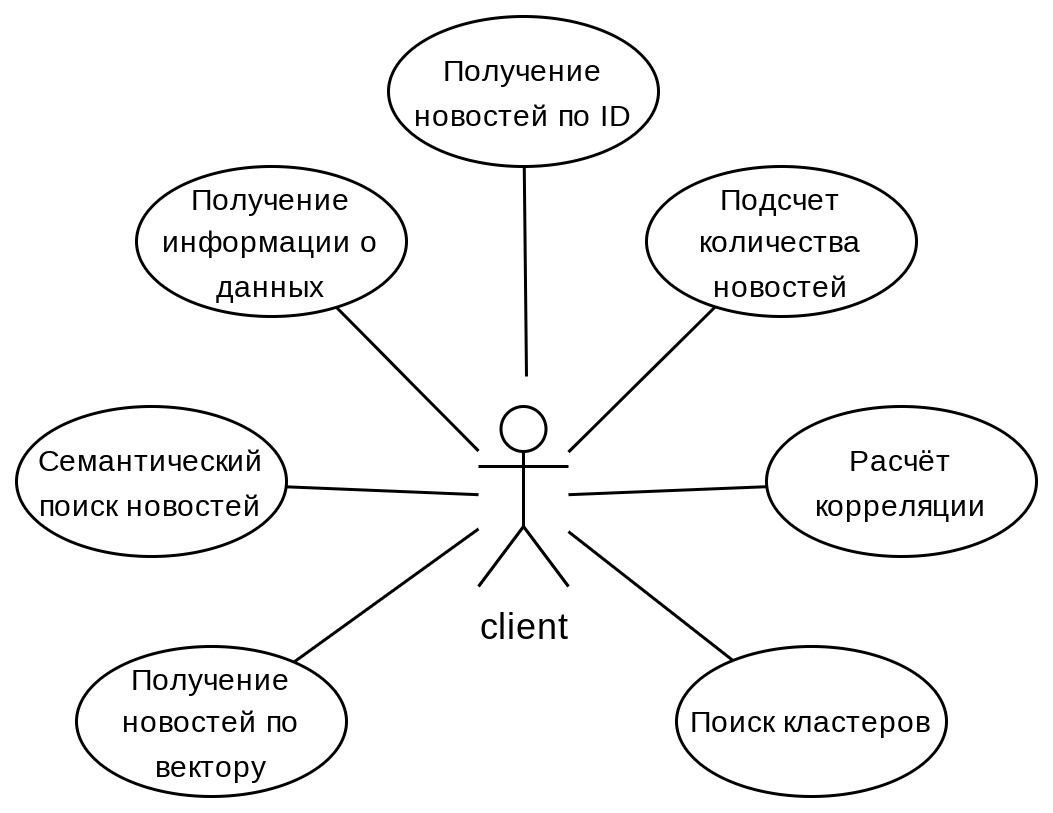
\includegraphics[width=\linewidth]{images/use-case-diagram.png}
    \caption{Диаграмма прецедентов системы}
    \label{img:use-case-diagram}
\end{figure}

Прецедент 1: Получение информации о данных.

Пользователь запрашивает информацию о датасете. В результате пользователь получает общую информацию о новостях: дату первой и последней новости в датасете, общее количество новостей.

Прецедент 2: подсчет количества новостей.

Пользователь запрашивает количество новостей. Для этого в запросе пользователь указывает обязательные параметры: границы временного интервала. Дополнительно пользователь может указать список интересующих тем новостей. В результате пользователь получает количество новостей за указанный временной интервал для каждой запрошенной темы (если они были представлены) и общее количество новостей за указанный временной интервал.

Прецедент 3: расчёт корреляции.

Пользователь запрашивает расчёт корреляции между количеством новостей и предоставленным пользователем временным рядом. Для этого пользователь указывает обязательные параметры: границы временного интервала, длительность окна, интересующую тему и список ~-- пользовательский временной ряд. В результате пользователь получает временной ряд ~-- корреляцию между количеством новостей и пользовательским временным рядом для каждого окна.

Прецедент 4: поиск кластеров.

Пользователь запрашивает кластеризацию новостей, т.е. определение основных тем новостей. Для этого пользователь указывает обязательные параметры: границы временного интервала. Дополнительно пользователь может указать параметры для алгоритма кластеризации. В результате пользователь получает список кластеров. Каждый кластер содержит список новостей, входящих в кластер.

Прецедент 5: Получение новостей по ID.

Пользователь запрашивает новость по ее ID. Для этого пользователь указывает обязательный параметр: ID новости. В результате пользователь получает данные о новости: ID, заголовок, дату и время публикации новости.

Прецедент 6: Получение новостей по вектору.

Пользователь запрашивает поиск ближайших новостей к заданному вектору. Пользователь указывает обязательные параметр: вектор и максимальное количество новостей, либо certainty для ограничения количества новостей. В результате пользователь получает список новостей, наиболее близких к указанному вектору. Каждая новость представлена следующими данными: ID, заголовком, датой и временем публикации новости.

Прецедент 7: Семантический поиск новостей.

Пользователь осуществляет семантический поиск новостей, т.е. получение новостей, наиболее близких к указанному текстовому запросу. Пользователь указывает обязательные параметр: текст запроса и максимальное количество новостей, либо certainty для ограничения количества новостей. В результате пользователь получает список новостей, наиболее близких к указанному запросу. Каждая новость представлена следующими данными: ID, заголовком, датой и временем публикации новости.

\section{Проектирование системы хранения данных}
Исходя из требований к сервису и пользовательских сценариев требуется определять извлекать из базы данных новости, относящиеся к определенным темам, задаваемым пользователем. Невозможно вручную разметить все новости, тем более, определить соответствие произвольным пользовательским запросам, поэтому необходимо применять методы машинного обучения для извлечения новостей, семантически близких к пользовательским запросам.

Для этого необходимо решить две задачи:
\begin{itemize}
    \item определение семантической близости новостей к запросу;
    \item извлечение некоторого количества самых семантически близких к запросу новостей.
\end{itemize}

Как было рассмотрено в главе 1, для решения задачи определения семантической близости текстовой информации применяются различные эмбеддинги.

Имея векторное представление новостей и векторное представление пользовательского запроса, задача определения наиболее семантически близких новостей сводится к задаче поиска ближайшего соседа.

В случае, если количество элементов, среди которых осуществляется поиск ближайших соседей, невелико, то могут применяться такие хорошо известные алгоритмы, как KNN (метод k-ближайших соседей). В противном случае, если имеется очень большое количество элементов, требуется применение особых алгоритмов, которые позволяют решать эту задачу эффективно.

Это семейство алгоритмов называется ANN (approximate nearest neighbor), и существует ряд алгоритмов для решения этой задачи. В качестве примера можно привести библиотеку FAISS [\textbf{TODO:ссылка}], которая реализует несколько быстрых алгоритмов ANN.

Тем не менее, использование библиотеки FAISS не всегда удобно, потому что она является низкоуровневой библиотекой, предоставляющей базовую функциональность. При использовании хранилища данных к нему выдвигаются такие требования, как
\begin{itemize}
    \item поддержка CRUD (create, read, update, delete) операций ~-- хранилище данных должно эффективно реализовывать эти операции, потому что в случае с большим объемом данных перестройка всего индекса (как это было бы в случае с непосредственным применением FAISS) на каждую операцию модификации данных привела бы к крайней низкой производительности системы;
    \item поддержка горизонтальной масштабируемости ~-- хранилище должно обеспечивать возможность репликации на несколько узлов вычислительной системы для увеличения производительности, если производительности одного узла не хватает для обработки запросов с требуемой задержкой;
    \item поддержка классических операций поиска и фильтрации ~-- помимо операций поиска ближайших соседей в векторном пространстве, хранилище данных должно поддерживать выполнение типичных операций баз данных, таких как фильтрация, сортировка итп;
    \item служебные возможности, такие как авторизация и контроль доступа.
\end{itemize}

Для решения всех этих задач служит особый класс баз данных ~-- векторные базы данных также называемые векторными поисковыми движками. Эти системы представляют собой нереляционные базы данных, которые способны осуществлять операции поиска с учетом близости векторного представления хранимых данных.

Векторные базы данных применяются для решения таких задач, как
\begin{itemize}
    \item семантический поиск ~-- поиск документов (например, веб-страниц) не по совпадению ключевых слов, а по семантической близости; иными словами, с помощью векторных поисковых движков можно найти документ, релевантный запросу, даже если он не содержит слова, используемые в запросе;
    \item поиск похожих изображений, например, идентификация человека по лицу.
\end{itemize}

Таким образом, было решено использовать векторную базу данных в качестве основы для разрабатываемой в рамках данной работы системы, потому что использование текстовых эмбеддингов совместно с векторной базой данных позволяет извлекать из базы данных новости, относящиеся к определенным темам, задаваемым пользователем.

\subsection{Выбор векторной базы данных}

\textbf{<TODO: обзор существующих векторных БД>}

Таким образом, было решено использовать векторную базу данных Weaviate для использования в разрабатываемой в рамках данной работы системы.

\section{Проектирование общей структуры системы}

Рассмотрим архитектуру системы анализа новостей и основные компоненты, из которых она состоит. Диаграмма архитектуры представлена на рисунке \ref{img:system-architecture}.

\begin{figure}[h]
    \centering
    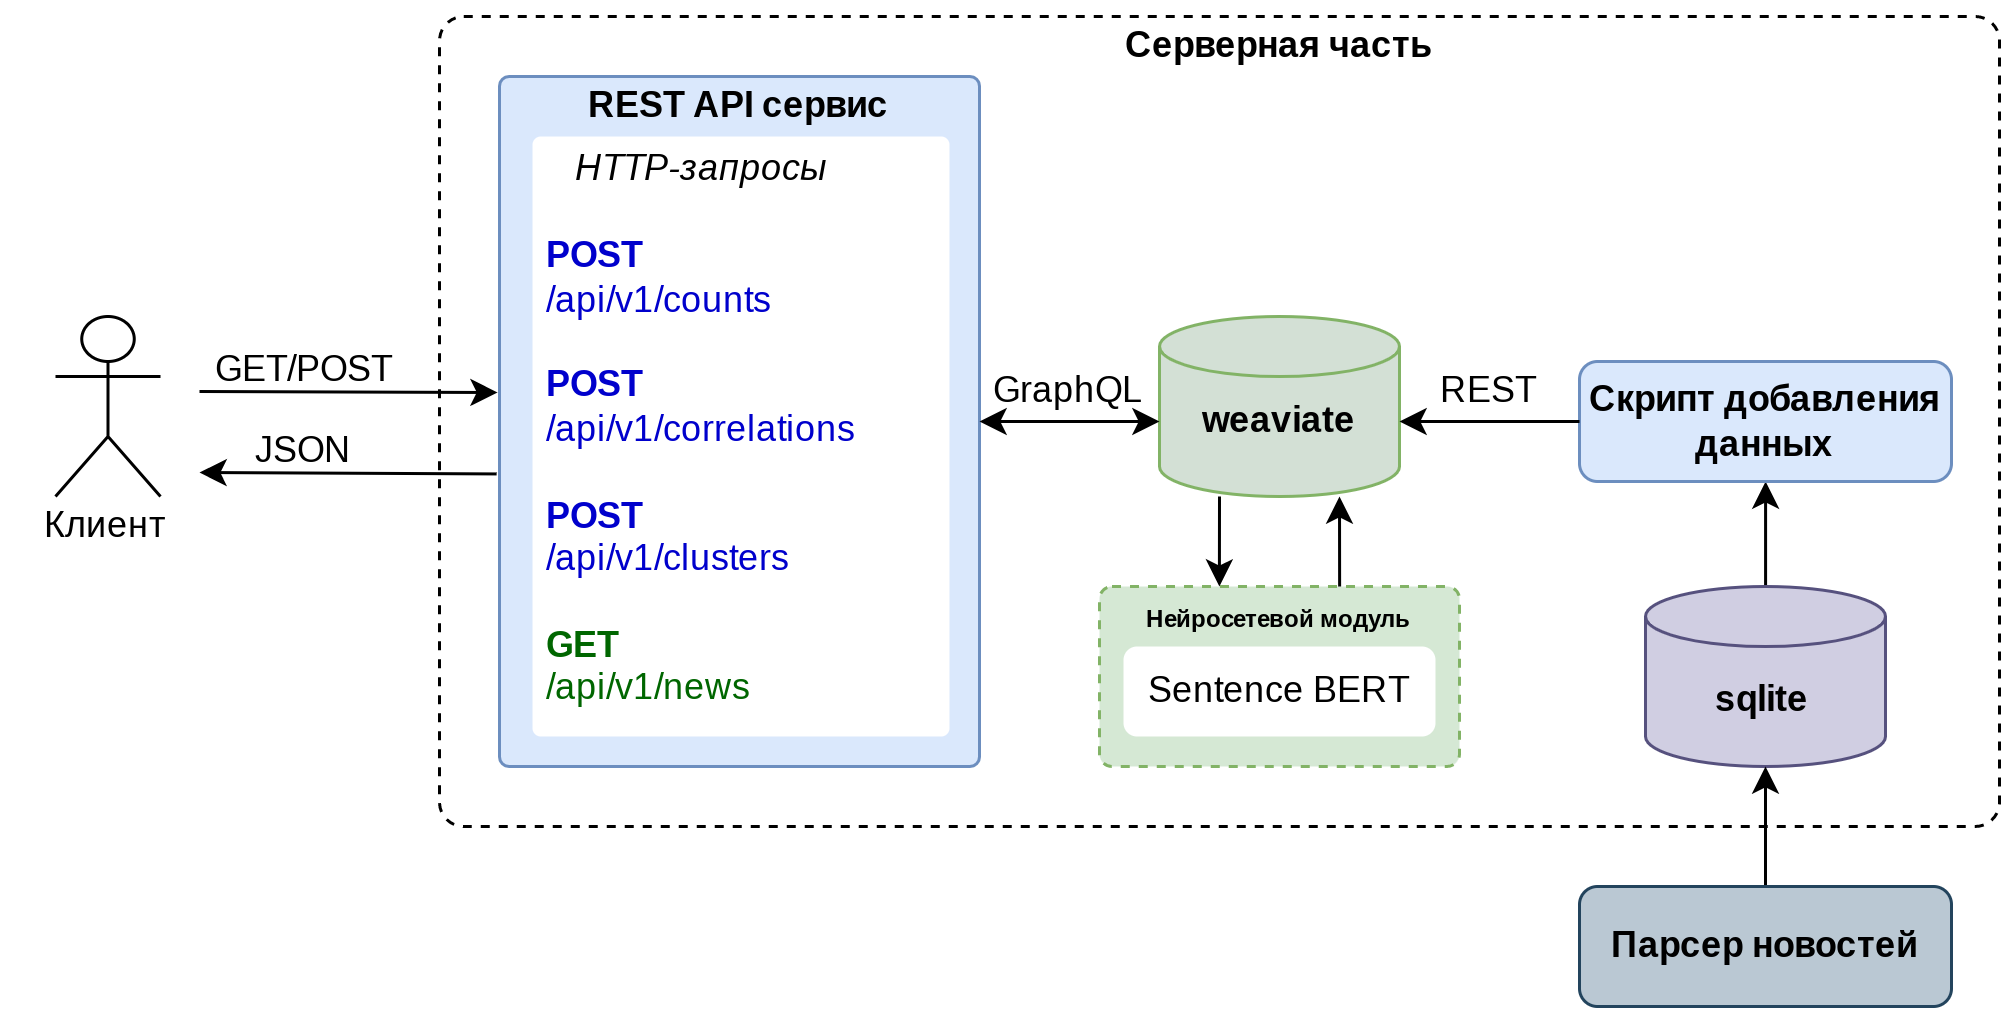
\includegraphics{images/system-architecture.png}
    \caption{Архитектура системы анализа новостей}
    \label{img:system-architecture}
\end{figure}

В основе системы, как было рассмотрено ранее, лежит векторная база данных Weaviate. weaviate выступает в качестве основного хранилища новостей и в качестве векторного поискового движка, который используется для извлечения новостей, относящиеся к определенным темам, задаваемым пользователем.

Для работы векторного семантического поиска, данные необходимо векторизовать. Для векторизации данных в Weaviate используются внешние модули. В данном случае, применяется стандартный модуль tex2vec-transformers, который осуществляет векторизацию текста с помощью нейронных сетей с архитектурой Трансформер.

Система представляет собой RESTful сервис, таким образом, необходим модуль, осуществляющий взаимодействие с клиентами с помощью REST. Этот модуль предоставляет внешнее REST-API сервиса и реализует основную логику сервиса, выполняя такие задачи как поиск новостей, расчет кросс-корреляции, кластеризацию новостей и другие. Для получения данных сервис обращается к базе данных Weaviate, используя язык запросов к данным GraphQL.

Для упрощения развертывания сервиса на узлах вычислительного кластера, применяются Docker контейнеры. Основные компоненты системы: Weaviate, модуль векторизации Weaviate и сервис развернуты в отдельных Docker-контейнерах.

В дополнении к рассмотренным компонентам системы, которые используются для функционирования сервиса, имеется подсистема получения новостей. Подсистема получения новостей используется для парсинга, обработки и сохранения новостей с целью дальнейшего использования сервисом. Подсистема получения новостей состоит из следующих компонентов:
\begin{itemize}
    \item парсер новостей ~-- скрипт, который непрерывно читает и сохраняет новости в sqlite базу данных;
    \item sqlite база данных ~--- промежуточное хранилище считанных новостей;
    \item скрипт для добавления данных переносит новости из промежуточного хранилища в sqlite в Weaviate; в процессе добавления новостей в БД Weaviate, происходит их векторизация.
\end{itemize}

\chapter{РАЗРАБОТКА И ТЕСТИРОВАНИЕ}
\aftertitle

\section{Выбор стека технологий}

Перед началом разработки системы анализа новостей был произведен анализ различных технологий и выбор стека технологий для разработки сервиса. Выбор основного компонента сервиса ~-- векторной базы данных ~-- был осуществлен в главе \ref{chap:arch_design}.

\subsection{Выбор языка программирования}

В качестве языка программирования для разработки системы анализа новостей был выбран Python. Выбор Python в качестве основного языка программирования для разработки системы анализа новостей обусловлен несколькими важными причинами.

Python является лидирующим языком в области науки о данных и машинного обучения. Большинство библиотек для этих задач написаны на Python или имеют привязки к нему.

Python является простым и высокоуровневым языком, который позволяет разрабатывать сложные системы, затрачивая меньше усилий, по сравнению со многими другими языками. : Python отличается от других языков своей простотой и читаемостью. Это ускоряет процесс разработки, облегчает отладку и поддержку кода.

Векторная база данных Weaviate, которая используется в этом проекте, имеет официальную клиентскую библиотеку для Python. Это обеспечивает удобный и надежный доступ к функциям базы данных.

Python имеет множество фреймворков для разработки веб-сервисов, таких как FastAPI, Flask и Django, что делает его идеальным выбором для создания веб-сервиса, предусмотренного в этом проекте.

\subsection{Выбор фреймворка для создания REST API}

Для реализации веб-сервиса нужно выбрать какой-либо фреймворк для разработки веб-приложений. В данной работе необходимо реализовать RESTful-сервис. Были сформулированы следующие требования к фреймворку:
\begin{itemize}
    \item поддержка реализации REST API;
    \item простота разработки и минимальное количество шаблонного кода;
    \item поддержка валидации входящих данных;
    \item поддержка создания документации в формате swagger.
\end{itemize}


Выбор подходящего фреймворка для реализации REST API в веб-сервисе зависит от многих факторов. Были рассмотрены преимущества и недостатки Django, Flask и FastAPI для данного проекта.

Django ~-- это высокоуровневый фреймворк разработки веб-приложений на Python, который обеспечивает полный набор функциональности "из коробки". Django предлагает ряд модулей для различных задач, включая аутентификацию, формы, маршрутизацию, управление сессиями и взаимодействие с базами данных. Django следует принципу DRY (Don't Repeat Yourself) и призывает к максимальному повторному использованию кода.

Преимущества:
\begin{itemize}
    \item обширная функциональность: Django имеет встроенные модули для работы с базами данных, административную панель, систему шаблонов и многое другое, что позволяет сократить время разработки;
    \item большое сообщество пользователей, что позволяет получить поддержку и множество ресурсов для изучения.
\end{itemize}

Недостатки:
\begin{itemize}
    \item избыточность: Django ~-- фреймворк, предназначенный для создания крупных веб-приложений со множеством функций, которые избыточны для REST сервиса;
    \item отсутствие некоторых функций для работы с REST API, таких как поддержки валидации данных и автоматической генерации документации Swagger.
\end{itemize}

Flask ~-- это фреймворк для разработки веб-приложений на Python. Он предназначен для создания небольших и простых веб-сайтов и API. В отличие от Django, Flask не предлагает множество функций "из коробки", но предоставляет основу, на которой можно строить, используя расширения. Flask предлагает больше гибкости, позволяя разработчикам выбирать инструменты и библиотеки, которые они хотят использовать.

Преимущества:
\begin{itemize}
    \item гибкость и модульность: Flask позволяет выбирать и использовать только те компоненты, которые действительно необходимы для проекта;
    \item простота использования: Flask легко изучить и начать использовать, особенно для небольших проектов.
\end{itemize}

Недостатки:
\begin{itemize}
    \item при создании REST API с Flask может потребоваться больше шаблонного кода по сравнению с другими фреймворками.
    \item отсутствие встроенной валидации данных, что может усложнить процесс разработки REST API.
\end{itemize}

FastAPI ~-- это современный, высокопроизводительный веб-фреймворк для построения API с Python. Он обеспечивает автоматическую генерацию документации для API, валидацию данных с помощью Python Type Hints и поддерживает асинхронные запросы. FastAPI был разработан с упором на удобство использования и производительность.

Преимущества:
\begin{itemize}
    \item FastAPI обеспечивает высокую производительность.
    \item встроенная валидация данных: FastAPI поддерживает валидацию данных на основе Python type hints, что облегчает проверку входящих данных.
    \item автоматическая генерация документации Swagger: FastAPI автоматически генерирует документацию Swagger на основе кода, что облегчает создание и поддержку документации API.
\end{itemize}

Недостатки:
\begin{itemize}
    \item FastAPI наименее популярный фреймворк, имеющий меньшее количество обучающих материалов.
\end{itemize}

Исходя из рассмотренных преимуществ и недостатков, для разработки проекта был выбран фреймоврк FastAPI. Он обеспечивает быстродействие и простоту использования, встроенную валидацию данных и генерацию документации Swagger, что полностью соответствует требованиям к фреймворку для этого проекта.

\section{Разработка системы добавления данных в векторную БД}

С помощью парсера новостные данные собираются и сохраняются в базе данных SQLite. Чтобы работать с ними, их необходимо проанализировать, очистить от выбросов и добавить в векторную базу данных Weaviate.

Были разработаны скрипты: скрипт для анализа и предобработки данных и скритпт для добавления новостей в Weaviate.

Для анализа и предобработки данных использовался язык программирования Python и библиотеки pandas, numpy и matplotlib. Это широко распространенные инструменты, применяемые в Data Science и при работе с данными, которые позволяют быстро выполнять множество различных операций, связанных с анализом и предобработкой данных.

В первую очередь, требуется определить временные рамки собранных новостей. В рамках работы, были собраны новости с 2019-04-23 по 2020-12-07. Т.к. собрано небольшое количество данных с новостных лент, то не представляет трудностей считать все данные в оперативную память и удобным образом работать с ними, используя средства библиотеки pandas, такие как DataFrame.

Следующим этапом предобработки является определение количества новостей за каждый день. Это позволит выявить ошибки и аномалии в данных.  До определенной даты, количество новостей существенно меньше, чем после этой даты. Изначально собиралось по несколько новостей, максимум, десятков новостей в день. Затем собирались от тысячи до двух тысяч новостей в день. Такая большая разница в количестве новостей в день может привести в дальнейшем к нарушению работы алгоритмов машинного обучения и к проблемам в определении корреляции новостей и тех или иных данных. Поэтому в рамках предобработки данных, необходимо удалить данные о новостях, относящиеся к периоду, в течении которого собиралось мало новостей в день

Обработанные данные сохранялись в промежуточный файл CSV.

Следующим этапом, эти данные из CSV файла считываются и добавляются в Weaviate. Предварительно, удаляется схема данных и все данные, чтобы избежать дублирования при повторном выполнении скрипта. Затем происходит создание схемы данных согласно \ref{chap:data-scheme}. После этого осуществляется последовательное добавление всех новостей в базу данных. Этот процесс занимает продолжительное время, потому что в момент добавления записей в базу происходит их векторизация с помощью указанного векторизатора (tex2vec-transformers с моделью MiniLM) и сохранение полученных векторов в базе.

Для работы с базой данных использовался официальная библиотека Weaviate для Python. Эта библиотека позволяет использовать все возможности базы данных, отправлять запросы на получение и модификацию данных с помощью Python без необходимости вручную работать с HTTP запросами REST и GraphQL.

\section{Разработка сервиса}

Для упрощения разработки и поддержки, весь код проекта разбит на модули. В процессе разработки сервиса была создана следующая структура файлов.
\begin{lstlisting}
service/
|-- app/
|-- scripts/
|-- main.py
\end{lstlisting}

В директории app находятся основные модули проекта. В директории scripts находятся вспомогательные скрипты, такие как скрипт добавления данных в базу данных Weaviate. Файл main.py является точкой входа в приложение, реализующей REST API с помощью фреймворка FastAPI. В main.py происходит обработка запросов, а основная логика выполнения запроса, например, обращение к БД, расчёт корреляции и т.п. осуществляется модулями из директории app.

Далее приведен пример обработки запроса поиска новостей с помощью семантического поиска:
\begin{lstlisting}
@app.get('/news')
def search_news(q: str):
    news = news_search.by_query(q)
    response = {
        'news': news
    }
    return response
\end{lstlisting}

С помощью декоратора определяется HTTP метод и URL конечной точки API, в данном случае, это GET и адрес "/news". Данная функция будет вызвана при получении соответствующего запроса. Параметры функции определяют параметры HTTP запроса. С помощью python type hints указывается тип параметра q: строка. В обработчике запроса происходит вызов функции семантического поиска новостей news\_search.by\_query(), которая возвращает список новостей, полученных из БД, близких к указанному запросу. Затем происходит формирование структуры и возврат ответа. FastAPI автоматически преобразует объект словаря в JSON и отправляет ответ пользователю.

\subsection{Разработка расчёта корреляции}

TODO: Написать про разработку механизма расчета корреляции

\subsection{Разработка метода определения основных новостей}

TODO: Написать про разработку кластеризации новостей для определения основных тем в заданном промежутке времени.


\section{Развертывание}

TODO: Написать про Docker


> Для упрощения развертывания сервиса на узлах вычислительного кластера, применяются Docker контейнеры. Основные компоненты системы: Weaviate, модуль векторизации Weaviate и сервис развернуты в отдельных Docker-контейнерах.

\chapter{НАУЧНАЯ СОСТАВЛЯЮЩАЯ}
\label{chap:research}
\aftertitle

В этой главе рассматривается экспериментальная работа по проверке разработанного сервиса и анализу новостей с его помощью. Описаны проведенные эксперименты по анализу новостей.

В исследовании использовались исторические данные новостей, собранные за 2020 год.

\section{Анализ количества новостей}

В первую очередь был произведен анализ количества новостей в день за исследуемый промежуток времени. На рисунке \ref{img:news-count} представлен график количества новостей за день. Минимальное количество новостей в день 165, максимальное ~-- 2890, а среднее ~--- 1907.

\begin{figure}[h]
    \centering
    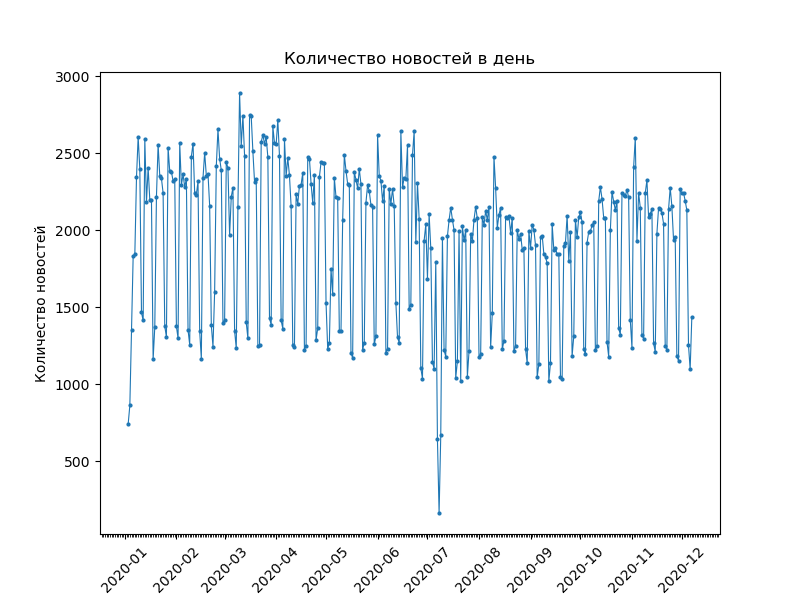
\includegraphics[width=\linewidth]{images/news-count.png}
    \caption{Количество новостей в день}
    \label{img:news-count}
\end{figure}

\section{Исследование расстояния между новостями}

Была изучена статистика попарного косинусного расстояния между векторным представлением новостей за день.

Косинусное расстояние двух векторов $a$ и $b$ ~-- это метрика схожести двух ненулевых векторов, определяемая как косинус угла между ними (\ref{eq:cosine-dist}).

\begin{equation}
    cos(\theta) = \frac{\vec{a} \cdot \vec{b}}{||\vec{a}|| \cdot ||{b}||}
    \label{eq:cosine-dist}
\end{equation}

Таким образом, эмбеддинги близких по смыслу новостей будут представлять собой два вектора с приблизительно одинаковым направлением, и их косинусное расстояние будет близко к единице. Наоборот, эмбеддинги противоположных по смыслу новостей будут представлять собой два вектора, направленные в противоположенные стороны, и их косинусное расстояние будет близко к минус единице. Таким образом, чем ближе косинусное расстояние к единице, тем более похожи новости.

Так как косинусное расстояние между векторным представлением соответствует семантической близости новостей друг другу, то статистика попарных расстояний может отражать характер распределения новостей по темам. Если за выбранный временной интервал много новостей на различные, то косинусное расстояние между ними будет близко к -1, и статистика попарных расстояния будут сдвинута в сторону меньших значений. Наоборот, если новости за выбранный временной интервал были на схожие темы, то косинусное расстояние будет близко к 1 , и статистика распределения попарных расстояний будет сдвинута в сторону больших значений.

На рисунке \ref{img:distances-distribution} показано сравнение распределения попарных косинусных расстояний за два дня. Распределение в области малых значений, т.е. новостей, которые не похожи друг на друга, совпадает. Различие наблюдается в области больших значений, т.е. новостей, которые похожи друг на друга. За один день наблюдается большее значение плотности распределения в области больших значений, чем за другой день, что говорит о том, что в этот день было больше новостей на близкие темы.

\begin{figure}[h]
    \centering
    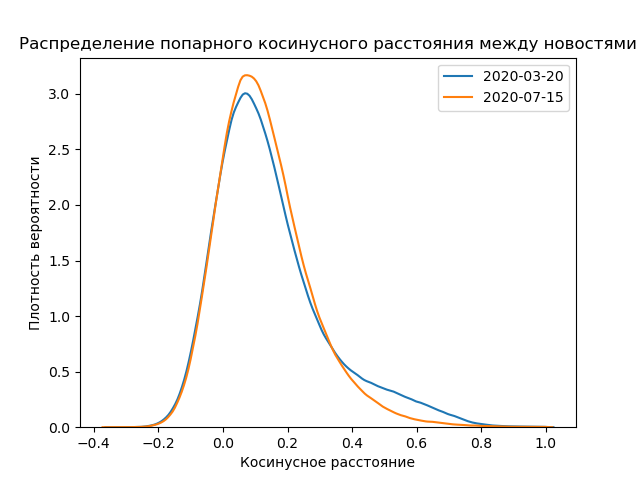
\includegraphics[width=\linewidth]{images/distances-distribution.png}
    \caption{Сравнение распределение косинусного расстояния между новостями за два дня}
    \label{img:distances-distribution}
\end{figure}

Так как построение распределения для всех дней не является наглядной визуализацией, то для изучения динамики изменения распределения попарных косинусных расстояний межу новостями, было решено построить графики отдельных квантилей: 50\% (медиана), 75\% и 90\%. График изменения распределения попарного косинусного расстояния по дням представлен на рисунке \ref{img:distances}.

\begin{figure}[h]
    \centering
    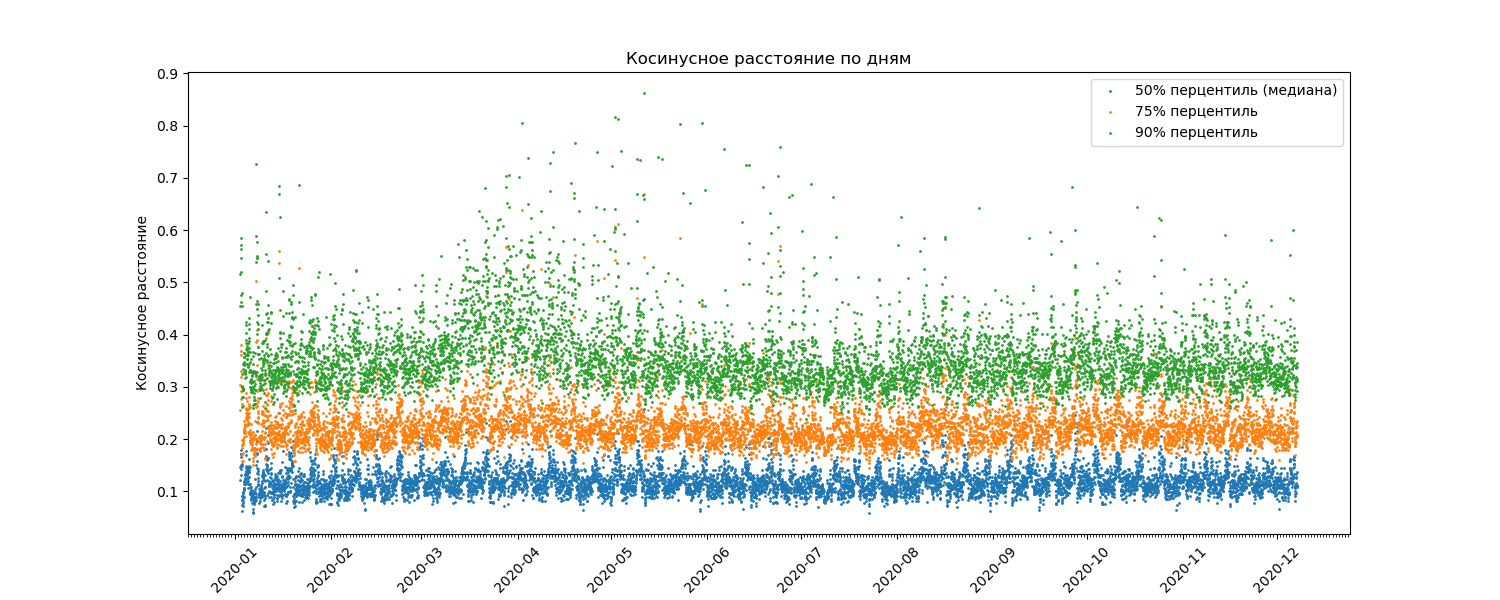
\includegraphics[width=\linewidth]{images/distances.png}
    \caption{Изменение распределения попарного косинусного расстояния по дням}
    \label{img:distances}
\end{figure}

На этом графике показаны значения трех квантилей: 50\% (синий), 75\% (оранжевый) и 90\% (зеленый) в виде точек. Каждая точка показывает значение соответствующего квантиля распределения попарного косинусного расстояния между новостями за один день. На графике мы  можем отчетливо видеть колебания с периодом 7 дней, по всей видимости, связанные с недельными изменениями в  распределении тематик новостей.

Значения 50\% квантиля практически не изменяются во времени, не считая недельных колебаний. Это согласуется с рассмотренным ранее на рисунке \ref{img:distances-distribution} сравнением распределения попарных косинусных расстояний между новостями за два дня, на котором видно, что в области малых значений распределение практически совпадает. Медианное значение 50\%-квантиля составляет 0.12, что соответствует непохожим новостям. Таким образом, распределение непохожих новостей мало меняется во времени, что может говорить о том, что в новостях всегда (за исключением недельных колебаний) охватывается примерно одинаково широкий круг тем.

Поведение значения 75\% квантиля мало отличается от поведения значений 50\% квантиля, но в них наблюдается небольшое увеличение в определенные моменты времени.

Наибольший интерес представляет поведение 90\% квантиля. Среди этих значений недельные колебания не так выражены, но выражен значительный рост значений в определенный период времени. Это говорит о том, что в этот момент времени распределение попарных косинусных расстояний между новостями было смещено в область больших значений, т.е. было больше новостей на похожие темы. По времени этот момент совпадает с началом пандемии коронавируса, карантина и экономического кризиса. Вероятно, эти темы обсуждались более активно, чем другие, что вызвало появление большего количества новостей на сходные тематики и смещение распределения попарного косинусного расстояния между новостями.

Таким образом, исследование распределения попарного косинусного расстояния между новостями может служить инструментом для выявления периодов с активным обсуждением тех или иных тем. При этом, наибольший интерес представляют больше квантили, такие как 90\%-квантиль.

\section{Исследование кросс-корреляции с финансовым инструментом}

Реализованный в данной работе сервис позволяет оценивать корреляцию количества новостей по заданным темам с различными временными рядами. В качестве примера, была изучена кросс-корреляция количества новостей по различным темам с ценой финансового инструмента ~-- с курсом доллара по отношению  к рублю, чтобы изучить, как разработанный сервис может быть использован в исследованиях финансовых рынков.

Для этого использовалось API сервиса /api/v1/correlations. С помощью этого API определялось количество новостей по заданным темам за данные промежутки времени и рассчитывалась корреляция с курсом доллара. Количество новостей определялось за окно длительностью 7 дней, которое сдвигалось с шагом 6 часов. Такое окно было выбрано, чтобы сгладить недельные колебания в количестве новостей.

Анализировалась корреляция абсолютного количества новостей с курсом доллара, корреляция относительного количества новостей с курсом доллара и корреляция абсолютного количества новостей с производной курса доллара.

\subsection{Корреляция количества новостей с курсом доллара}

Для исследования были выбраны следующие темы, которые могли бы быть актуальны на исследуемый период: экономика, политика, коронавирус, самоизоляция, курс доллара, фондовый рынок, нефть, кризис, акции.

Перед расчётом кросс-корреляции, значение количества новостей и стоимости доллара нормировались таким образом, чтобы попасть в диапазон $[-1; 1]$. Нормировка осуществлялась с помощью класса MinMaxScaler из библиотеки scikit-learn.

Графики корреляции количества новостей по темам "нефть" и "коронавирус" приведены на рисунке \ref{img:correlation-absolute}. На верхних половинах графиков показаны нормированные значения количества новостей (оранжевый) и курса доллара (синий). На нижних половинах графиков показано значение корреляционной функции (синий).

По данным графикам затруднительно сделать какие-либо выводы о влияние изменения стоимости финансового инструмента на новости и наоборот.

\begin{figure}[h]
    \centering
    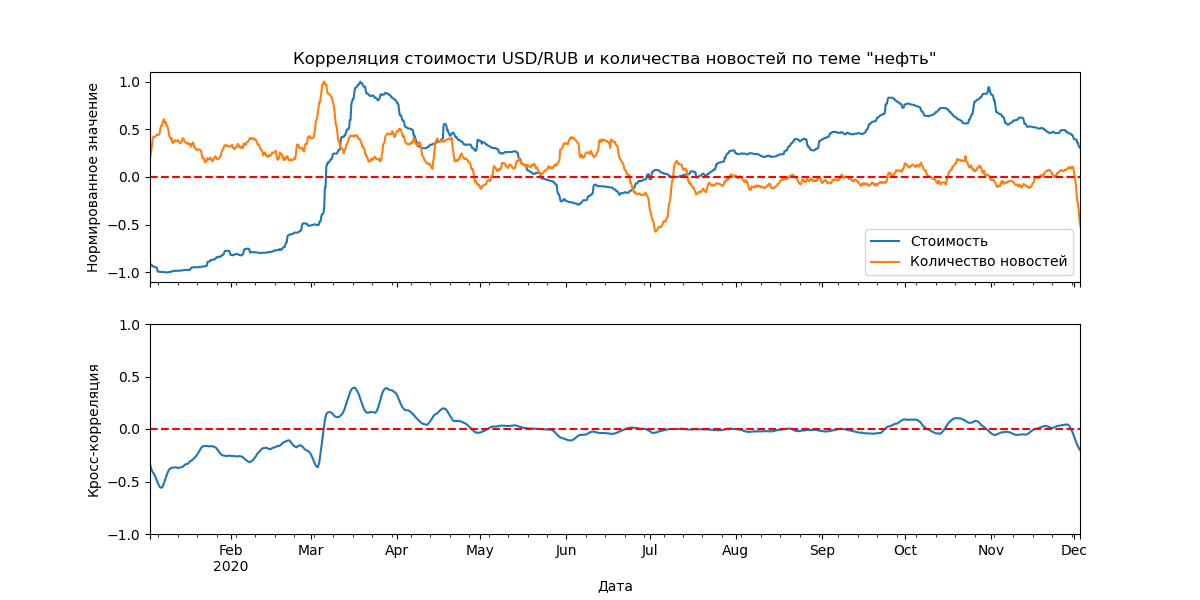
\includegraphics[width=\linewidth]{images/correlations/absolute/нефть.png}
    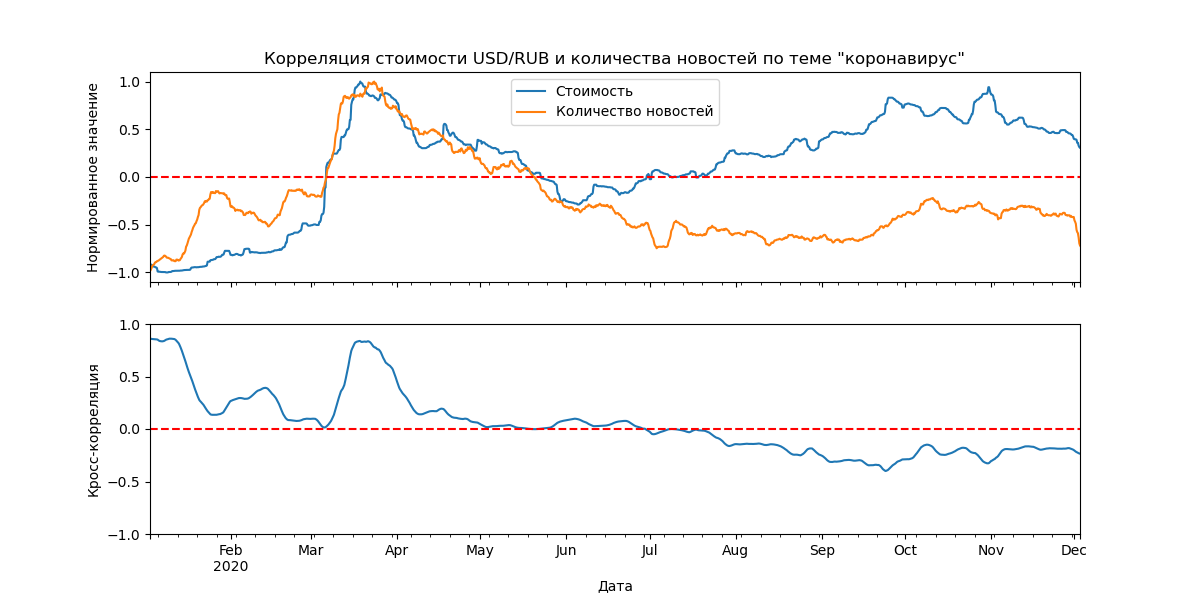
\includegraphics[width=\linewidth]{images/correlations/absolute/коронавирус.png}
    \caption{Корреляция количества новостей по различным темам с курсом доллара}
    \label{img:correlation-absolute}
\end{figure}


\subsection{Корреляция относительного количества новостей с курсом доллара}

Рассмотрим аналогичные графики, но для относительного количества новостей. Количество новостей по той или иной теме было нормировано на общее количество новостей за день, чтобы не учитывать влияние количества новостей, а только относительную долю рассматриваемой теме в общем количестве новостей за заданный временной интервал.

Графики корреляции относительного количества новостей по темам "нефть" и "коронавирус" приведены на рисунке \ref{img:correlation-relative}. На верхних половинах графиков показаны нормированные значения количества новостей (оранжевый) и курса доллара (синий). На нижних половинах графиков показано значение корреляционной функции (синий).

По данным графикам затруднительно сделать какие-либо выводы о влияние изменения стоимости финансового инструмента на новости и наоборот.

\begin{figure}[h]
    \centering
    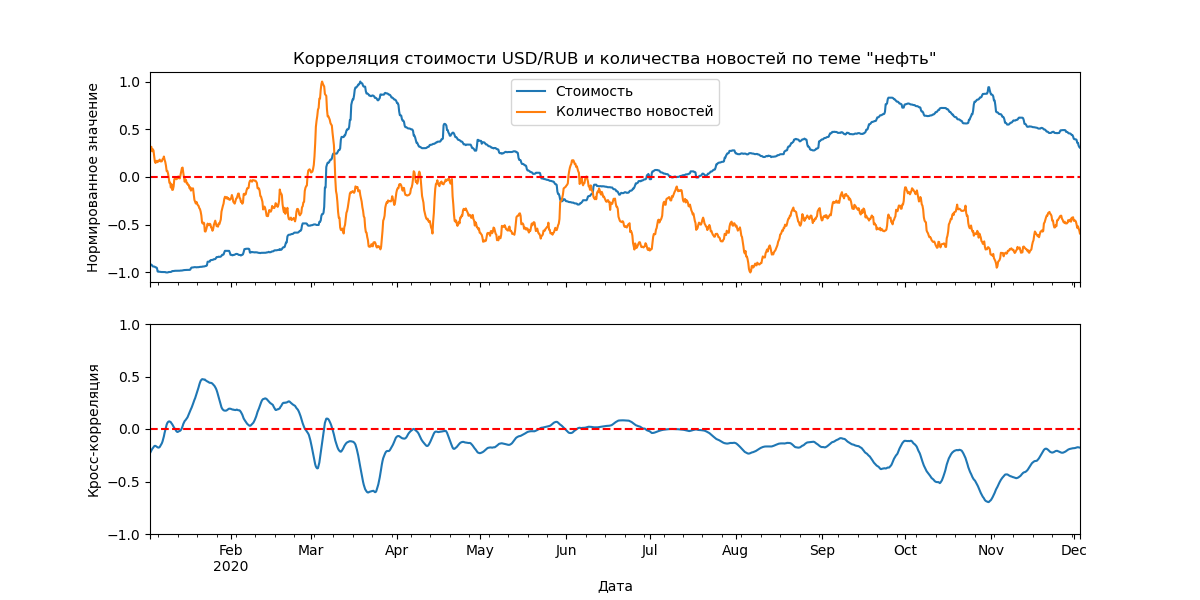
\includegraphics[width=\linewidth]{images/correlations/relative/нефть.png}
    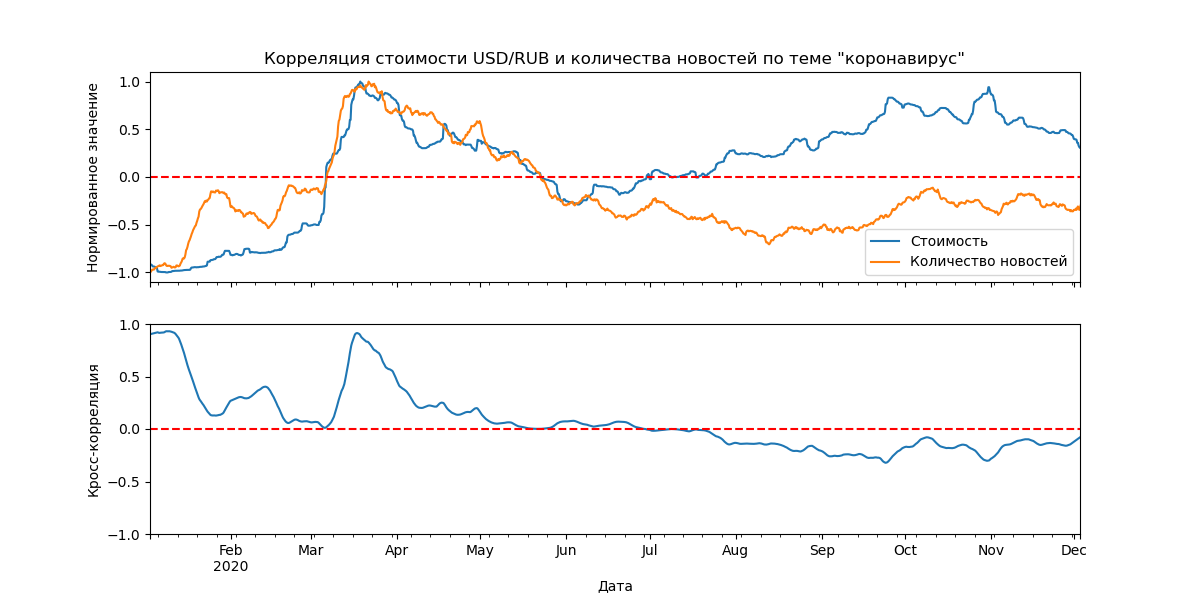
\includegraphics[width=\linewidth]{images/correlations/relative/коронавирус.png}
    \caption{Корреляция относительного количества новостей по различным темам с курсом доллара}
    \label{img:correlation-relative}
\end{figure}

\subsection{Корреляция количества новостей с производной курсом доллара}

Было выдвинуто предположение, что в новостях отражается не сколько сам курс доллара, сколько его изменения. В периоды, когда курс доллара приблизительно стабилен, это не находит активного отражения в новостях. В периоды, когда происходят сильные колебания курса доллара, это находит активное отражение в новостях, как в специализирующихся на экономике изданиях, так и в общих средствах массовой информации.

Для того, чтобы проанализировать корреляцию количества новостей с изменениями курса доллара, курс доллара был численно дифференцирован. Для дифференцирования применялась центральная разностная схема (\ref{eq:derrivative}). Регулируя параметр шага можно влиять на сглаженность производной. Т.к. курс доллара имеет множество мелких колебаний, то для анализа только крупных изменений, шаг дифференцирования может быть увеличен.

\begin{equation}
    C'_i \approx \frac{C_{i+n} - C_{i-n}}{2n}
    \label{eq:derrivative}
\end{equation}
\noindent\begin{tabularx}{\linewidth}{lllX}
    где & $C_i$    &~--& стоимость в момент времени $i$, \\
        & $i$      &~--& момент времени, \\
        & $n$      &~--& шаг. \\
\end{tabularx}

На рисунке \ref{img:usd_derrivative} показан курс доллара (верхний) и производная курса доллара (нижний) за рассматриваемый период.

\begin{figure}[h]
    \centering
    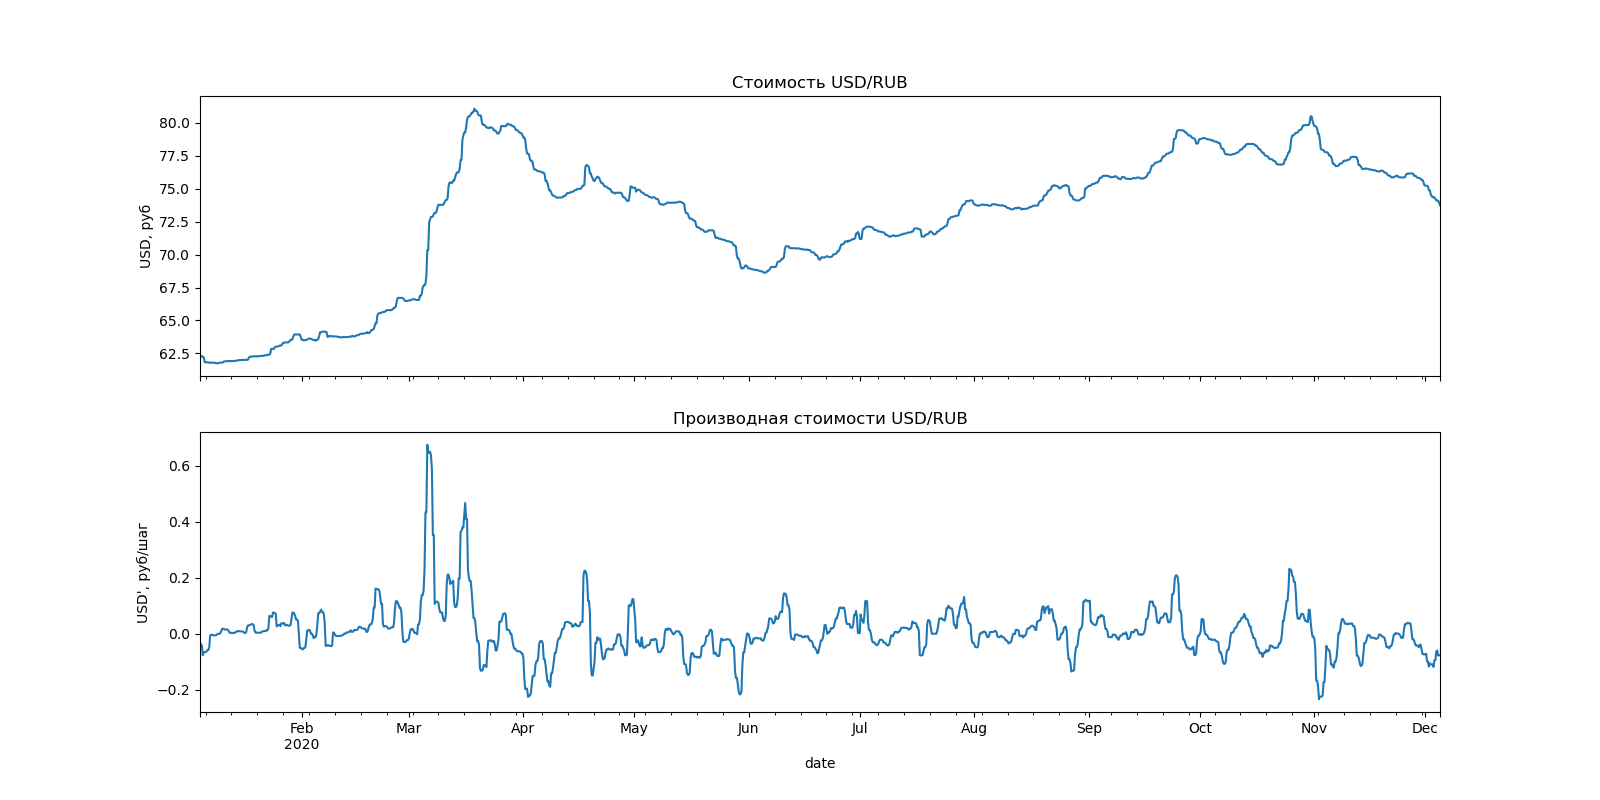
\includegraphics[width=\linewidth]{images/correlations/usd_derrivative.png}
    \caption{Производная курса доллара}
    \label{img:usd_derrivative}
\end{figure}

Для расчёта корреляции необходимо нормализовать данные. Но для производной курса доллара MinMaxScaler не подходит, потому что при его применении может произойти сдвиг нуля, а нуль имеет важное значение для производной курса, обозначая отсутствие изменений. Поэтому, был применен другой способ нормализации, который масштабирует размах функции в интервал $[-1; 1]$, но сохраняет положение нуля (\ref{eq:derr-normalize}). Данный способ определяет максимальный размах значения функции от нуля и масштабирует ее таким образом, чтобы максимальный размах составлял единицу.

\begin{equation}
    \begin{array}{l}
        k = max(max(C'), -min(C')), \\
        C'_{norm} = k \cdot C'
    \end{array}
    \label{eq:derr-normalize}
\end{equation}\noindent\begin{tabularx}{\linewidth}{lllX}
    где & $C'$         &~--& производная стоимости, \\
        & $C'_{norm}$  &~--& нормированная производная стоимости. \\
\end{tabularx}


Используя рассмотренный способ нормализации, была рассчитана корреляция между количеством новостей по определенным темам и производной курса доллара.

Графики корреляции относительного количества новостей по темам "нефть" и "коронавирус" приведены на рисунке \ref{img:correlation-derrivative}. На верхних половинах графиков показаны нормированные значения количества новостей (оранжевый) и курса доллара (синий). На нижних половинах графиков показано значение корреляционной функции (синий).

\begin{figure}[h]
    \centering
    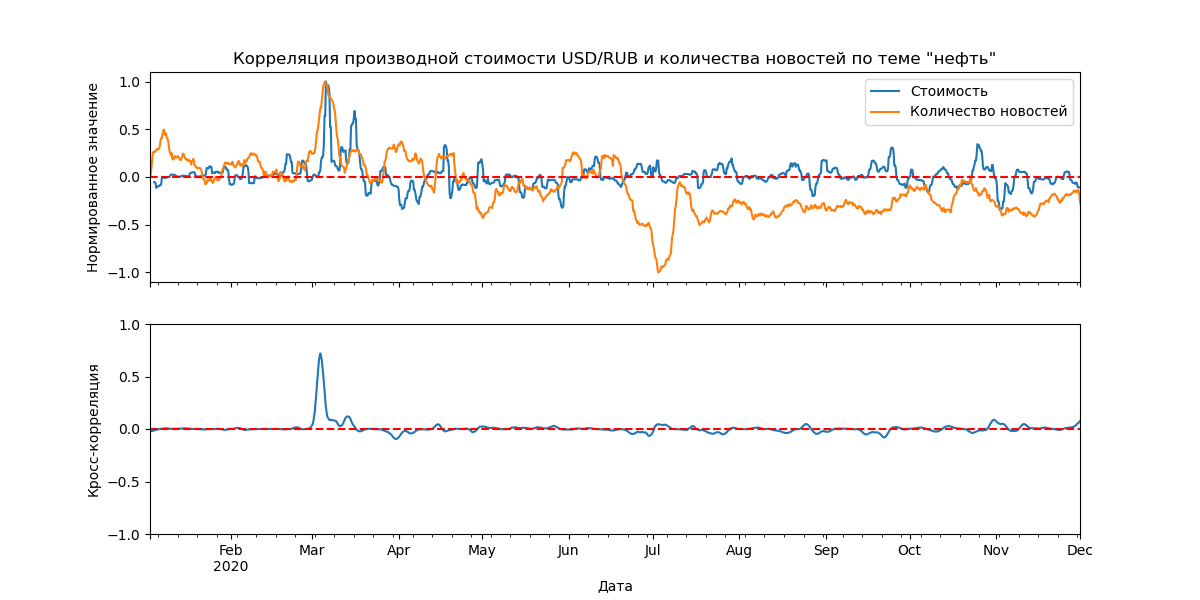
\includegraphics[width=\linewidth]{images/correlations/derivative/нефть.png}
    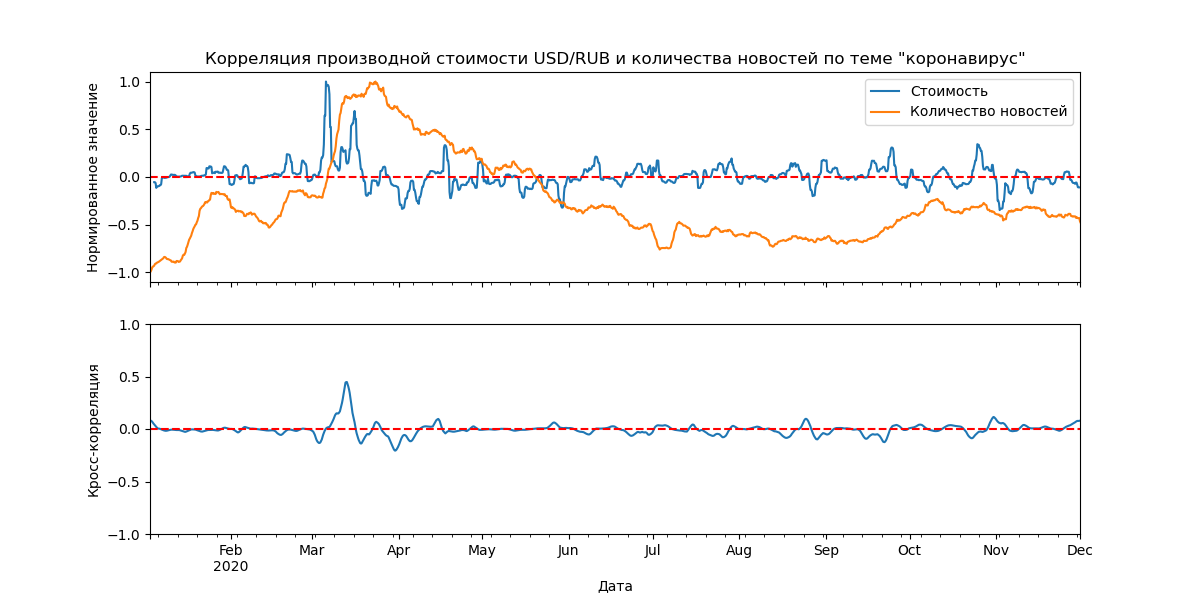
\includegraphics[width=\linewidth]{images/correlations/derivative/коронавирус.png}
    \caption{Корреляция количества новостей по различным темам с производной курса доллара}
    \label{img:correlation-derrivative}
\end{figure}

Использование производной курса доллара позволило улучшить результаты. Теперь на графиках корреляции отчетливо видны моменты корреляции сильных изменений курса и обсуждений определенных тем, в то время как в остальные моменты времени значение корреляции около нуля.

\nnchapter{ЗАКЛЮЧЕНИЕ}

В результате проведенной работы был спроектирован и реализован RESTful сервис для анализа новостей. Сервис позволяет осуществлять семантический поиск новостей, определять количество новостей по различным темам, рассчитывать корреляцию количества новостей по определенной теме с различными временными рядами и осуществлять определение популярных новостей с помощью кластеризации.

Основная область применения разработанной системы ~-- социальные, финансовые и маркетинговые исследования, выявление трендов и их взаимосвязи.

Сервис был развернут на персональном компьютере с ОС Linux с графическим ускорителем NVidia RTX 3060. База данных Weaviate и модуль векторизации текстов с помощью нейронных сетей были развернуты в Docker-контейнерах с помощью docker compose, а сервис и вспомогательные инструменты запускаются на хосте.

В ходе работы были проведены исследования по анализу новостей с помощью разработанной системы.

Было исследовано изменение распределения попарных косинусных расстояний между новостями и было установлено, что в моменты крупных событий (таких как кризис и пандемия), 90\%-квантиль распределения сдвигается в сторону больших значений, что может быть использовано для определения детектирования событий.

Была исследована корреляция количества новостей по определенным темам и стоимости финансового инструмента. Обнаружена корреляция количества новостей, связанных с экономикой с сильными колебаниями курса доллара. Это позволяет использовать разработанный сервис как для экономических исследований, таких как исследование отражения тех или иных событий в медиа, так и, возможно, для краткосрочного прогнозирования стоимости финансовых инструментов.

Была рассмотрена кластеризация новостей и было показано, что с помощью кластеризации новостей можно объединять похожие новости в группы.


\newpage
\let\oldthepage=\thepage  % Сохранить нумерацию
\renewcommand{\thepage}{} % Убрать номера страниц
\printbibliography[title=СПИСОК ИСПОЛЬЗОВАННЫХ ИСТОЧНИКОВ]
\newpage
\let\thepage=\oldthepage  % Восстановить нумерацию

\end{document}
